%%%%%%%%%%%%%%%%%%%%%%%%%%%%%%%%%%%%%%%%%%%%%%%%%%%%%%%%%%%%%%%%%%%%%%%%%%%%%%%%
%2345678901234567890123456789012345678901234567890123456789012345678901234567890
%        1         2         3         4         5         6         7         8

\documentclass[letterpaper, 12 pt, conference]{ieeeconf}  % Comment this line out
                                                          % if you need a4paper
%\documentclass[a4paper, 10pt, conference]{ieeeconf}      % Use this line for a4
                                                          % paper

\IEEEoverridecommandlockouts                              % This command is only
                                                          % needed if you want to
                                                          % use the \thanks command
\overrideIEEEmargins
% See the \addtolength command later in the file to balance the column lengths
% on the last page of the document

\usepackage[utf8]{inputenc}
\usepackage[T1]{fontenc}
\usepackage{graphicx}

% The following packages can be found on http:\\www.ctan.org
%\usepackage{graphics} % for pdf, bitmapped graphics files
%\usepackage{epsfig} % for postscript graphics files
%\usepackage{mathptmx} % assumes new font selection scheme installed
%\usepackage{mathptmx} % assumes new font selection scheme installed
%\usepackage{amsmath} % assumes amsmath package installed
%\usepackage{amssymb}  % assumes amsmath package installed

\title{\LARGE \bf
Music Genre Classification of Closely Related Sub-Genres 
}

\author{ \parbox{2 in}{\centering Chris Calloway
        \thanks{*Use the $\backslash$thanks command to put information here}\\
        Electrical Engineering\\
       Stanford University\\
        {\tt\small cmc2374@stanford.edu}}
        \hspace*{ 0.5 in}
        \parbox{2 in}{ \centering Yiwen Jiang
        \thanks{**The footnote marks may be inserted manually}\\
        Electrical Engineering \\
        Stanford University\\
        {\tt\small yjiang98@stanford.edu}}
          \hspace*{ 0.5 in}
        \parbox{2 in}{ \centering Louise Zhuang
        \thanks{**The footnote marks may be inserted manually}\\
        Electrical Engineering \\
        Stanford University\\
        {\tt\small @stanford.edu}}
}

% \author{ Chris Calloway$^{1}$, Yiwen Jiang$^{2}$, Louise Zhuang$^{3}$% <-this % stops a space
% \thanks{* Supervised by Mert Pilanci, Yifei Wang}% <-this % stops a space
% \thanks{$^{1}$ Chris Calloway
%         {\tt\small cmc2374 at stanford dot edu}}%
        
% \thanks{$^{2}$ Yiwen Jiang
%         {\tt\small  at stanford dot edu}}%

% \thanks{$^{3}$ Louise Zhuang
%         {\tt\small  at stanford dot edu}}%
        
    
% }


\begin{document}



\maketitle
\thispagestyle{empty}
\pagestyle{empty}


%%%%%%%%%%%%%%%%%%%%%%%%%%%%%%%%%%%%%%%%%%%%%%%%%%%%%%%%%%%%%%%%%%%%%%%%%%%%%%%%
\begin{abstract}

This report presents our attempt at training a model to predict music sub-genre labels of closely related musical genres. Musical genres, at their core, are subjective categorical labels based on human perception and consensus. Yet musical genre classification using broader genres (such as rap, rock, classical and jazz) has had much success in the machine learning community. Our goal was to see if such methods could extend to closely related genres to either find the existence (or lacktherof) of a distinction between closely related genres which we call sub-genres.




\end{abstract}


%%%%%%%%%%%%%%%%%%%%%%%%%%%%%%%%%%%%%%%%%%%%%%%%%%%%%%%%%%%%%%%%%%%%%%%%%%%%%%%%
\section{INTRODUCTION}

\subsection{Overview}

Music genres are subjective labels critics and consumers alike put on music for categorization purposes. 
As a consequence of this subjectivity, the labeling of genres is often controversial and a point of discussion among musical groups. 

Nonetheless, to a lay observer, what distinguishes rock and roll music from classical music is sonically and empirically obvious. Thus it isn't terribly surprising that machine learning methods applied to the classification of music to broad musical categories (rap, rock and roll, classical, jazz, etc) yields results in excess of 89 \% \cite{c1} \cite{c2} \cite{c3}. Thus despite the subjectivity of music labels, there is enough data within audio samples for both humans and machines alike to confidently classify music into broader genres.

But what about more closely related genres? In this paper we consider the rock and roll subgenres of Shoegaze and Dreampop. Fans and critics are split on what (if anything) defines the difference between the two genres. Is there enough evidence in the audio data to find such a distinction? 

A critical assumption we made before attempting to answer this question is that there is a ground truth sub genre label for these sub genres. That is, we take the genre, either "shoegaze" or "dreampop", that the artist's record label officially assigned to a particular album without regard to any fan or critical debate of the accurateness. We used a collection of these officially labeled "dreampop" or "shoegaze" albums from various artists and various record labels as our audio data for our training.

Our results indicate that with our assumption in place: 




\subsection{Related Work}


There has been lots of work in the field of music genre classification. As mentioned in the overview, the results of various machine learning classifiers is upwards of 89\%, with the best being the CNN such as \cite{c4}. 

There has been less work in looking at very niche sub-genre classification in particular. One such attempt was made to classify Metal Sub-genres in \cite{c5}. In this paper, 30 second samples of songs from sub genre specific Spotify playlists were taken for various metal sub-genres such as black metal and thrash metal. The audio data was then converted into Mel spectograms. This data was split into 80\% training data and 20\% testing data and then was fed into a Convolutional Recurrent Neural Network. After training, the network was able to predict metal sub-genres on the test set with a 62\% accuracy. 

In another paper, decision trees, random forests, extremely randomised trees, and gradient tree boosting were used to classify 23 EDM subgenres \cite{c6}. The authors were able to achive an accuracy of 59\% without any neural networks involved.

In another paper about classifying 3 subgenres of jazz, neural networks, linear SVM and KNN were used to classify the subgenres. The authors were able to achieve classification accuries of 79.39\%, 67.12\%, and 77.43\%  respectively \cite{c7}. The authors also found that adding a multi-layer perceptron network before a long term short memory layer in their neural netowork boosted the accuracy to 89.824\.%

From this related work, we concluded that while training a neural network looked promising in terms of getting the best results, we also found it necessary to train a KNN and SVM model given that they were likely to produce sufficient albeit perhaps sub par results. 




\section{PROCEDURE}


\subsection{Data collection}

To train our model we collected specifically genre labeled data from Spotify. 578 shoegaze songs and 577 dreampop songs, as labeled by the Record Label of their containing album, were collected and downloaded using the Spotify API.
The Spotify API only allows a random 30 seconds of the song to be downloaded so all such songs were 30 second samples taken at a random interval. When adding  songs, we added them by the entire album, only excluding songs that did not have 30 second samples or other such audio features and remixed songs from other artists if applicable.

Not all songs were strictly "dreampop" or strictly "shoegaze". For example some were labled as "dreampop and etheral pop" or "shoegaze and noise rock". We allowed for such genre blends in our dataset. However, an album that was labeled as "dreampop and shoegaze" was not allowed. We restricted our dataset to allow only one album per artist to encourage a varkety of artists in our database. To determine which album to add to the database we picked the earliest released album with the proper label. Note that in some cases an artist would have a release as "shoegaze" and perhaps later in their discography a release as "dreampop". We allowed for this, so in some cases an artist appears in both the shoegaze and the dreampop datasets with different albums. 

After the sample songs were downloaded, the mp3 data per genre was read and stored into on large matrix. This large and randomly split 70\% train samples and 30\% test samples. These samples were then stored in .npy files.

\subsection{Data Pre-processing and Feature Extraction}
From the .npy files the train and test data was read, converted into a Mels spectogram for the purpose of training Neural Network, then stored once again into respective train and test folders. An example spectogram for the dreampop song "Zebra" by Beachouse is shown below

The MFCC was also being extracted as features from each data sample for training the KNN and SVM model. MFCC (Mel-Frequency Cepstral Coefficients) is one of the most commonly used features for audio and speech recognition machine learning purposes. MFCC provides more reliable spectral estimations for audio signals compared to straightforward spectral transformations. 

The calculation of MFCC takes into account the characteristics of audio signals as well as human hearing. Since music genres are human perceived labels, such an audio feature was appropriate for our models. For MFCC, signals are framed into shorter frames to account for the fact of the constantly changing nature of audio signal. The calculation of power spectrum and use of Mel filter bank mimics human hearing where different emphasis is put on different ranges of frequencies. This is represented in wider bands used at higher frequencies, as the focus is on energy rather than variation, whereas it is the opposite for lower frequencies. The final coefficients are obtained through calculating the Discrete Cosine Transform coefficients of the logarithm of the filter bank energies. 

For our purpose, the original mp3 files were being read in with sampling rate of Fs = 22050, thus each 30 seconds data sample has length of 661500. Taking this into account 16 MFCCs are being used, with frame length of 2048 and hop length of 512. 

With the given MFCC feature parameters, for each audio sample, we obtain 16 MFCC with length of 1288. Using the output MFCC as is would result in heavy computational load. To reduce this load, the coefficients for each window were then flattened into a one-dimensional sequence, and principal component analysis (PCA) was performed to reduce the dimensionality of the data for better classification accuracy. PCA compresses data by maintaining feature information in the dimensions of highest variance, thus preserving key information about the Mel spectral features while also de-noising the data.


\begin{figure*}
  \includegraphics[width=\textwidth, height=6cm]{Screen Shot 2021-04-16 at 6.40.00 PM.png}
  \caption{Sample Spectogram}
\end{figure*}


\subsection{KNN Design}

\newline \,\,
\nelwine TODO: Talk about the design choices for making the KNN here
\newline \,\,

\subsection{SVM Design}
For this project with SVM, we focused on fitting processed data with linear model. A linear SVM has the goal of finding the hyperplane that produces the largest separation of margin between the categories. Two different optimization schemes Stochastic Gradient Descent (SGD) and Adaptive Moment Estimation (ADAM) were being used. Stochastic gradient descent reduces the computation load comparing to normal gradient descent by randomly selecting data points each time to calculate derivatives. Adam on the other hand, computes the adaptive learning rate for each parameters as well as storing average of past exponential decaying gradient. The hinge loss function shown below was used.\\
$L = \frac{1}{2} ||w||^2 + \frac{c}{n}\sum_{i=1}^{n}max(0,1-y_iw_ix_i) $\\
20 epochs with batch size of 30 was used. 

Linear SVM models were generated with all four databases, the hyperparameters including learning rate and C were being tuned. The loss vs. iteration as well as loss vs. accuracy graphs were being plotted and examined. 

\newline \,\,

\subsection{NN Design}

TODO: Talk about the design choices for making the NN here
\newline \,\,


\section{Results}

The results from training our model for KNN, SVM, and NN are shown below
\newline \,\,

\par KNN Results (probably don't need to split this in train/test (TODO FIX)

\begin{center}
    \begin{tabular}{ |c|c| }
 KNN Train & KNN Test  \\ 
 0\% & 0\% \\

\end{tabular}\\

\end{center}

\par TODO: Dicussion of KNN results
\newline \,\,


\par SVM results :\\
\quad While achieving similar maximum accuracy, the model generated with Adam optimization algorithm displayed a faster convergence in the loss function plot. Thus the result reported below are based on models generated using Adam optimization algorithm.

\begin{center}
    
    \begin{tabular}{ |c|c|c| }
 Subgenres & SVM Train & SVM Test \\ 
 Shoegaze vs Dreampop & 72.5\% & 74.5\% \\
 Progressive vs Math Rock & 69.3\% & 67.1\% \\
 Progressive vs Tech House & 65.4\% & 65.5\% \\
 Folk vs Roots Rock & 74.3\% & 65.3\% \\
\end{tabular}\\
\end{center}
\begin{figure}[t]
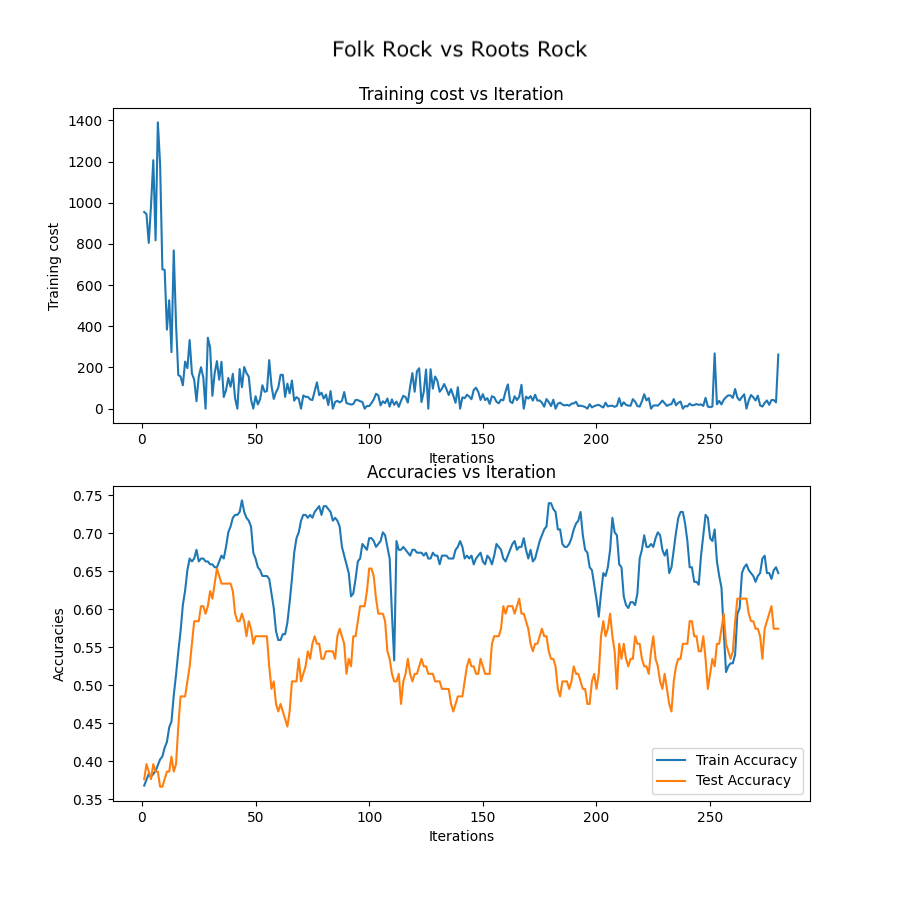
\includegraphics[width=8cm]{EE269 Project/frrr_svm.png}
\caption{Folk Rock vs Roots Rock}
\end{figure}
\begin{figure}
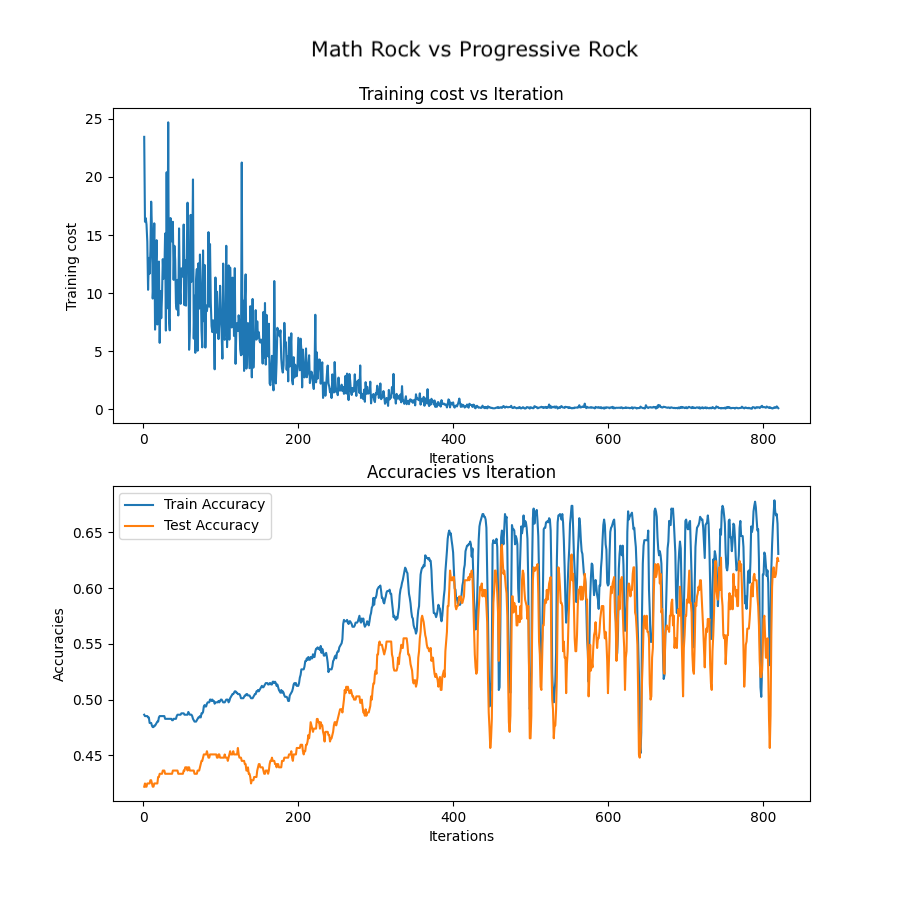
\includegraphics[width=8cm]{EE269 Project/mrpr_svm.png}
\caption{Math Rock vs Progressive Rock}
\end{figure}
\begin{figure}
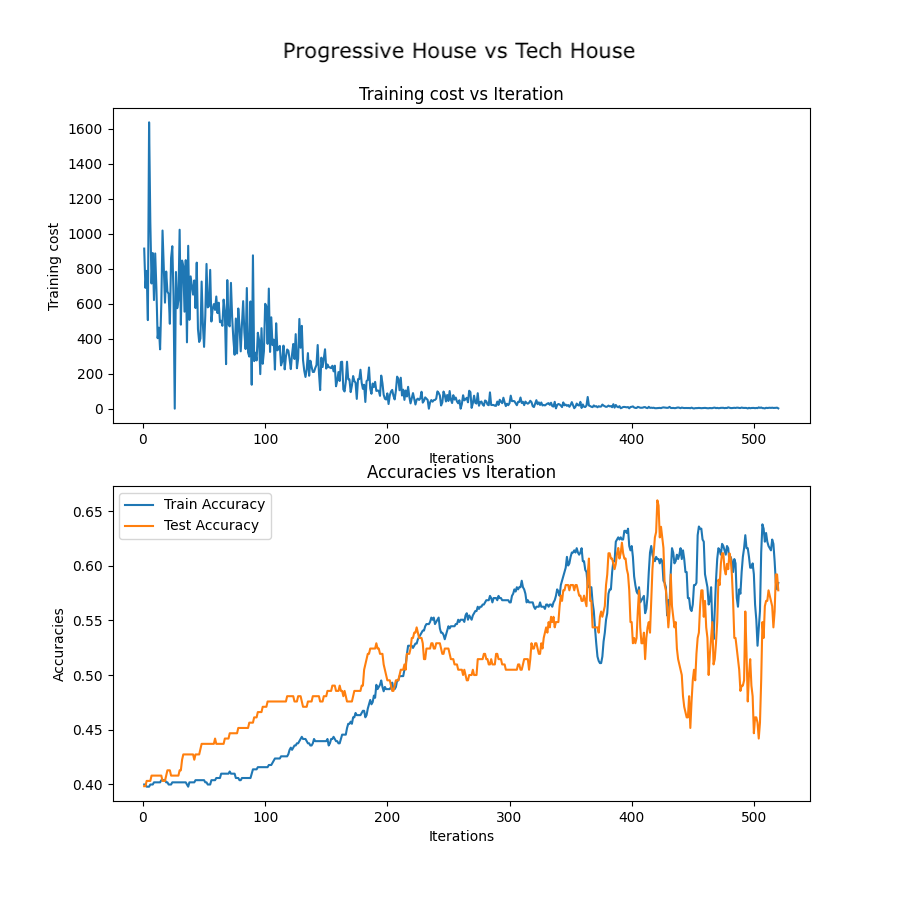
\includegraphics[width=8cm]{EE269 Project/phth_svm.png}
\caption{Progressive House vs Tech House}
\end{figure}
\begin{figure}
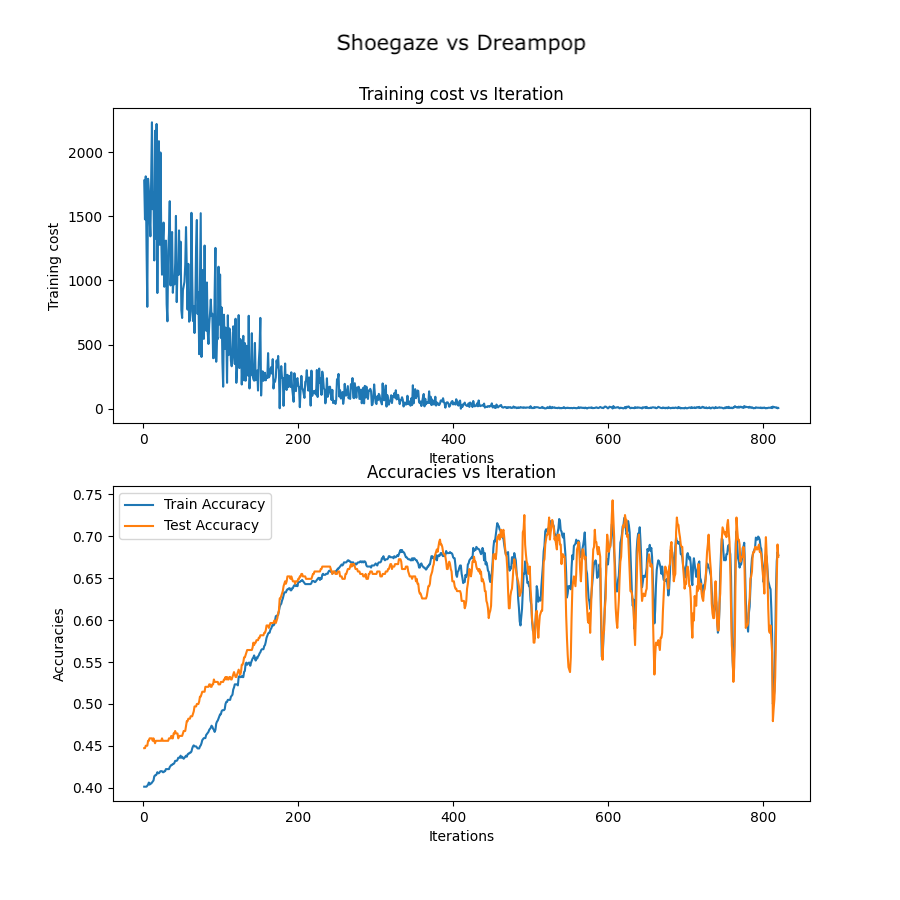
\includegraphics[width=8cm]{EE269 Project/sgdp_svm.png}
\caption{Shoegaze vs Dream pop}
\end{figure}

\par In general, the training and testing accuracy obtained with the data fitted with linear SVM models ranged from mid-sixties to mid-seventies. The model generated on the Shoegaze and Dreampop database demonstrated the highest accuracy. The accurcy of model on Progressive Rock and Math Rock, as well as Progressive House and Tech House are slightly lower. However, these results are expected as they are within the range to results shown in existing paper focusing on similar subject. Moreover, our project focused only on linear models, and existing papers have presented higher result when use other kernel for the SVM. 
\newline \,\,



\par Our NN results are as follows:
\begin{center}
    \begin{tabular}{ |c|c| }
 NN Train & NN Test \\ 
 0\% & 0\%  \\

\end{tabular}\\
\end{center}


\par TODO: Dicussion of NN results
\newline \,\,



 

\section{Discussion}

TODO: Dicussion of all results


\section{Conclusion}


TODO: Conclusion based on results



\section*{ACKNOWLEDGMENT}

The authors would like to thank Mert Pilanci and Yifei Wang for their guidance on this project



\begin{thebibliography}{99}



\bibitem{c1} Cataltepe, Z., Yaslan, Y. & Sonmez, A. Music Genre Classification Using MIDI and Audio Features. EURASIP J. Adv. Signal Process. 2007, 036409 (2007). https://doi.org/10.1155/2007/36409

\bibitem{c2} Bahuleyan, Hareesh. "Music genre classification using machine learning techniques." arXiv preprint arXiv:1804.01149 (2018)..

\bibitem{c3} Haggblade, Michael, Yang Hong, and Kenny Kao. "Music genre classification." Department of Computer Science, Stanford University (2011). 

\bibitem{c4} Choi, Keunwoo, et al. "Convolutional recurrent neural networks for music classification." 2017 IEEE International Conference on Acoustics, Speech and Signal Processing (ICASSP). IEEE, 2017.


\bibitem{c5} Montgomerie, Adam.  Music genre classification of mel-spectrograms using convolutional and
recurrent neural networks. 2020

\bibitem{c6}  Antonio Caparrini, Javier Arroyo, Laura Pérez-Molina & Jaime Sánchez-Hernández (2020) Automatic subgenre classification in an electronic dance music taxonomy, Journal of New Music Research, 49:3, 269-284, DOI: 10.1080/09298215.2020.1761399



\bibitem{c7} R. J. M. Quinto, R. O. Atienza and N. M. C. Tiglao, "Jazz music sub-genre classification using deep learning," TENCON 2017 - 2017 IEEE Region 10 Conference, 2017, pp. 3111-3116, doi: 10.1109/TENCON.2017.8228396.


\end{thebibliography}




\end{document}
